\documentclass[12pt]{report}
\usepackage[a4paper]{geometry}
\usepackage[utf8]{inputenc}
\usepackage[myheadings]{fullpage}
\usepackage{fancyhdr}
\usepackage{lastpage}
\usepackage{float}
\usepackage{graphicx, wrapfig, subcaption, setspace, booktabs}
\usepackage{graphicx}
\usepackage[T1]{fontenc}
\usepackage[font=small, labelfont=bf]{caption}
\usepackage{fourier}
\usepackage[protrusion=true, expansion=true]{microtype}
\usepackage[english]{babel}
\usepackage{sectsty}
\usepackage{url, lipsum}
\usepackage[T1]{fontenc}
\usepackage{icomma}
\usepackage{siunitx}
\usepackage{ragged2e}
\usepackage{amsmath}
\usepackage{comment}
\usepackage{textgreek}
\usepackage{fancyhdr}
\usepackage{lastpage}
 \usepackage{indentfirst}
\pagestyle{fancy}
\fancyhf{}

\rfoot{Page \thepage \hspace{1pt} of \pageref{LastPage}}


\newcommand{\HRule}[1]{\rule{\linewidth}{#1}}
\onehalfspacing
\setcounter{tocdepth}{5}
\setcounter{secnumdepth}{5}
\setcounter{section}{0}

%-------------------------------------------------------------------------------
% HEADER & FOOTER
%-------------------------------------------------------------------------------
\pagestyle{fancy}
\fancyhf{}
\setlength\headheight{15pt}
\fancyhead[L]{Michal Ormos}
\fancyhead[R]{CPME}
\fancyfoot[R]{}

\begin{comment}
-Udledninger
$$
\begin{aligned}


\end{aligned}
$$

-Opgavetekst
\begin{figure}[H]
\includegraphics[width=0.5\textwidth]{"path"}
\end{figure} 


-Opgave billede med tekst
\begin{figure}[H]
\caption{"Billedtekst"}
\includegraphics[width=0.5\textwidth]{"path"}
\end{figure} 

-Værdier
$\\

$


\end{comment}


\begin{document}

\title{ \normalsize \textsc{Universidad de Valladolid}
		\\ [2.0cm]
		\HRule{0.5pt} \\
		\LARGE \textbf{\uppercase{Parallel computing and emerging models}}
		\HRule{2pt} \\ [0.5cm]
		\normalsize \today \vspace*{5\baselineskip}}

\date{}

\author{
		Michal Ormos}

\maketitle
\newpage

\tableofcontents


%\chapter{Introduction}

%These papers is going to present and explain these parts:

\chapter{Distributed systems}
	\section{History}
		Over past 60 years, computing technologies had experienced many series of platform and environmental changes that were driven by rising demand of applications workload and large data sets. A result of this phenomenon was rising demand in every few decades. These effect occur both to hight performance computing (HPC) and hight throughput computing (HTC).
        These lead to changes in architecture, operating systems, platform and network connectivity.
        In early years only centralized system were used, which conclude in creating parallel and distributed computing systems. These systems became data-intensive and network-centric.
        
        In present years billions of people are connected to Internet every day. In these demands supercomputers and large data centers must provide high-performance computing service to huge number of Internet users connected at the same time. Because of that high-performance computing are no longer optimal method for measuring system performance. The emerge of clouds instead demands high-throughput computing (HTC).
        
	\subsection{High-Performance Computing (HPC)}
    	High Performance Computing most generally refers to the practice of aggregating computing power in a way that delivers much higher performance than one could get out of a typical desktop computer or workstation in order to solve large problems in science, engineering, or business.
    	
        HPC introduce first computing paradigm which empathize the raw speed performance in 1990s in Gflops to 2010  in Pflops. FLOPS represent number of floating point operations per second, which can be understand as a method of encoding real numbers within the limits of finite precision available in computers. Using floating-point encoding, extremely long numbers can be handled relatively easily. A floating-point number is expressed as a basic number or \textit{mantissa} , an \textit{exponent}, and a \textit{radix}(number base).
    
\begin{figure}[ht]
\centering
     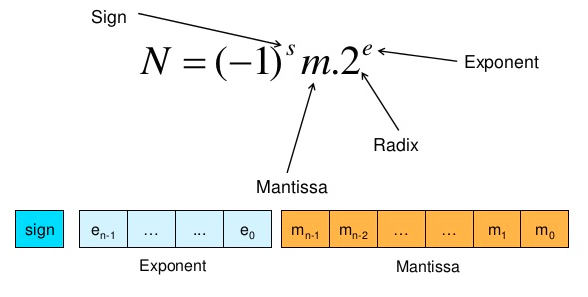
\includegraphics[width=0.5\textwidth]{img2.png}
      \caption{Explanation of FLOPS storing technique.}
       \label{img2}
\end{figure}    
            
    \subsection{High-Throughput Computing (HTC)}
	For many experimental scientists, scientific progress and quality of research are strongly linked to computing throughput. In other words, most scientists are concerned with how many floating point operations per month or per year they can extract from their computing environment rather than the number of such operations the environment can provide them per second or minute. Floating point operations per second (FLOPS) has been the yardstick used by most High Performance Computing (HPC) efforts to evaluate their systems. Little attention has been devoted by the computing community to environments that can deliver large amounts of processing capacity over long periods of time. We refer to such environments as High Throughput Computing (HTC) environments.\cite{htcondor}

	HTC paradigm pays more attention to high-flux computing, describing the use of many computing resources over long periods of time to accomplish a computational task.
\begin{figure}[ht]
\centering
     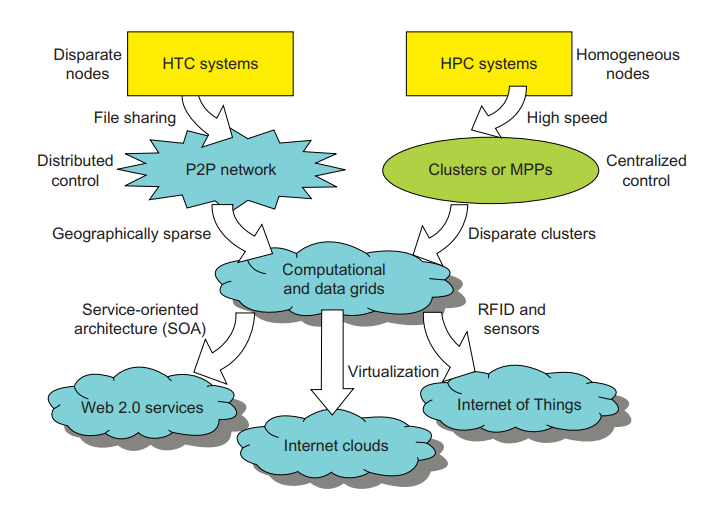
\includegraphics[width=0.7\textwidth]{img1.png}
      \caption{HPC vs. HTC diference throught history}
       \label{img1}
\end{figure} 
    
    \subsection{Computing paradigms}
    	In Figure \ref{img1} we introduced SOA. SOA is a style of applications architecture in such a way that they are composed of discrete software agents that have simple, well defined interfaces and are orchestrated through a loose coupling to perform a required function.
        As web 2.0 services, clouds and IoT which will be explained later.

Computing paradigm distinctions:
\begin{itemize}
\item \textbf{Centralized systems:}
        Every piece of the system is tight together in one place and accessed by terminal. Many data centers and supercomputers are
centralized systems, but they are used in parallel, distributed, and cloud computing applications.
\item \textbf{Parallel systems:}
        System is parallel connected together, many CPU's sharing one memory. An example of parallel computing would be two servers that share the workload of routing mail, managing connections to an accounting system or database, solving a mathematical problem etc.
\item \textbf{Distributed systems:}
        A distributed system is a network that consists of autonomous computers that are connected using a distribution middle-ware. They help each other in sharing different resources and capabilities to provide users with a single and integrated coherent network.
\item \textbf{Cloud:}
        Taking physical servers (WSC) and virtualized them to increase the number of accessible servers. This system is build on the idea that any of the servers is working full-time on 100\% and mostly is idle. Based on Quality of Service (QoS) and Service Level Agreement (SLA).
        Using idea of utility computing, which means charging the clients by the amount of energy they consume from the server, pay-as-you-go.
        Cloud can work as centralized or distributed system.
\end{itemize}

\subsection{Design objectives:}
\begin{itemize}
\item \textbf{Efficiency:}
	Level of accomplishment to use resources wisely.
\item \textbf{Dependability:}
	Reliability to provide high-throughput with Quality of Service (QoS). Guarantee that system will keep running or recover even under failure conditions.
\item \textbf{Adaptation:}
	Measures the ability to support billions of job requests
over massive data sets and virtualized cloud resources under various workloads and service
models.
\item \textbf{Flexibility:}
Measures the ability of distributed systems to run well in
both HPC (science and engineering) and HTC (business) applications.
\end{itemize}

\section{Scalable computing trends}
It's well know that Moore's law and other predictable trends in technology used tob drive computing applications further. It's not sure if it will continue.

Besides the Moore's law we record also Gilder's law which, likewise to Moore's law logic indicates that network bandwidth will double each year.

\subsection*{Degrees of Parallelism}
\textbf{Bit-level parallelism} (BLP) is the way of how historic big bulky computers were designed into bit-serial fashion over the years, user graduated from 4-bit microprocesors to 8-bit, 16-bit, 32-bit and now 64-bits CPUs.

This lead to next wave of improvement known as \textbf{instruction-level}, where the CPUs executes multiple instructions rather than only one instruction at a time, which later leads to pipeling, VLIW (very long instruction word) architectures, and multithreading requiring branch prediction, dynamic scheduling, speculation, and compiler support.%to work efficiently.

In that time \textbf{Data-level parallelism} (DLP) was made popular through SIMD (single instruction, multiple data) and vector machines using vectors. From ever since the introduction of multicore processors and chip multiprocessors (CMPs), we have been exploring \textbf{task-level parallelism} (TLP). Modern CPUs explores all of the parallelism types. As we move from parallel processing to distributed processing, we will see an increase in computing granularity to \textbf{job-level parallelism} (JLP).

Job-level brings the possibility of new applications as web services based on multiple tasks to provide complex services (maps, search, email) and Clusters service which is based on WSC (Warehouse-Scale Computers) Figure \ref{img2}. Innovative applications have different requirements than traditional. Hundreds of thousands of users scalability.

\begin{figure}[ht]
\centering
     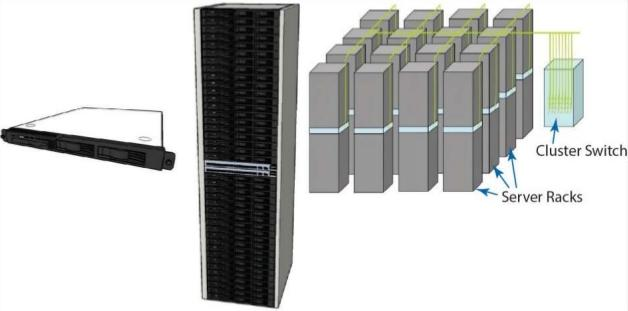
\includegraphics[width=0.7\textwidth]{img3.jpg}
      \caption{Sketch of the typical elements in warehouse. From (left) 1U server | (middle) 7' rack with Ethernet switch | (right) diagram of small clusters}
       \label{img2}
\end{figure}    

\subsection*{Hardware and Software}
Hardware of distributed systems was developing through years from single-core CPUs to Many-core CPUs, which lead to huge ability for instruction crunching - PFLOPS.

Many-core CPUs are usually partly GPU based, which can improve computing power.

\begin{figure}[ht]
\centering
     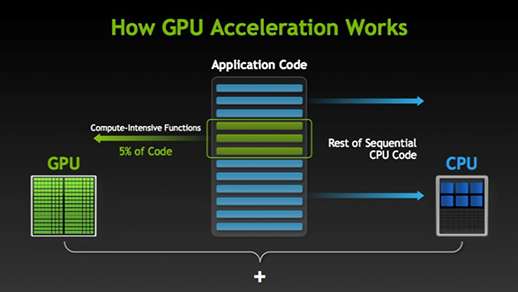
\includegraphics[width=0.7\textwidth]{img4.png}
      \caption{Diagram of how GPU can improve computing time of some operations, better than CPU \cite{nvidia}}
       \label{img4}
\end{figure}    

In case of Hardware also Simultaneous Multi-Threading (SMT) is used. SMT is a processor design that combines hardware multi threading with super-scalar processor technology to allow multiple threads to issue instructions each cycle.

In past years also memory as part of hardware was significantly improved mostly by increasing of capacity four times every three years. But access time didn’t significantly
changed over time. Which was caused by problems like memory walls and caches.

In case of solid disk capacity, we saw increasing by size, 10x every 8 years, but not increase by access time caused by mechanical hardware limits. Solid state disks (SSD) improve access time
but have a durability problem and still don't have enough inner space requirements for reasonably price.

By type the type saving the data, we distinguish Storage Area Network (SAN), where disk are unite with the given system that they are not accessible by other system. As second type we use Network Attached Storage (NAS), where disk are connected to the network, so they are accessible by the whole network of other systems and machines.

Software Service-Oriented Architecture (SOA) is style of software design where services are provided to the other sections by components of applications. Trough communication protocols. They are independent unit of functionality. A set of provided services become a software application.

Distributed operation systems is a software over a collection of heterogeneous OS platforms. Independent, network communicating, physically separate, middle-ware with a limited degree of resource sharing.

Parallel and distributed programming models contribute to computing scalability and flexibility. For example distributed shared memory, shared address space in threads or synchronization by messages. Performed by tools tests as MPI, MapReduce or Hadoop. For example Hadoop library by Yahoo allow write and run applications over vast amounts of distributed data.

\subsection*{Performance metrics and scalability analysis}
Are the ways of measuring the throughput of the system. Mostly used metrics nowadays are MIPS, TPS or already mentioned TFLOPS. Further metrics as job response time, latency, QoS etc.

System scalability can be amend by changing the size of machine, by software upgrades in OS or other OS components as libraries and software. Other ways for application scalability are matching the problem size scalability with machine size scalability or by technology as ability to adapt and fully use new core generations, new way of communication with hardware etc.

\subsection*{System availability} \label{MTTF}
Probability that a system will work as required during the period of a mission. Measured by Mean Time To Failure (MTTF) and Mean Time To Repair (MTTR).
\begin{equation}
System\quad availability = \frac{MTTF}{MTTF+MTTR}
\end{equation}
System availability can be improved by hardware redundancy, design of testability, component reliability etc.

\subsection*{Networks threats and data integrity}
Most of the systems are trying ensure security of their system by monitoring loss of confidentiality, integrity, system availability or inappropriate authentication. With right security approach and caution we can prevent this attacks.

\subsection*{Energy efficiency}
Energy consumption generate the most expensive part of server costs. We want to ensure that server are running and not just in idle condition, so we can maximally used components, which are defined by their lifetime. Further we apply energy-aware applications or middle-ware layer with energy-efficient techniques for task scheduling.

\subsection{Amdahl's and Gustafson's Law}
Amdahl's law is formula which can give theoretical speedup(S) in latency of the task execution time(\textalpha) at fixed workload(W) by number of processors(n)
\begin{equation}
S = \frac{1}{\alpha + \frac{1-\alpha}{n}}
\end{equation}

Gustafson's Law is formula which unlike of Amdahl's law give the theoretical speed at fixed execution time, which can be expected of a system whose resources are used.
W = workload of a given program with 1 processor; \textalpha = fraction of sequential code in W; W = workload scaled for n processors.
\begin{equation}
S' = \frac{\alpha W + (1 - \alpha )nW}{W}
\end{equation}

\chapter{Clusters}
Cluster is build of one or more computers, workstations, servers, blades, multi-core computers, etc. Possibly of different speeds and number of processors, called “nodes”, that are owned and managed by the same entity (a person, a group of people or a project) in which all the nodes run the same version of MOSIX and are configured to work tightly together.
Clusters have evolved to data centers and WSC, to later became the base for clouds.

In other words cluster is collection of stand-alone interconnected computers which work together as single computer resource. In this fashion cluster contain high potential of availability, scalability, tolerance of faults, modular growth and massive parallelism. Massively parallel processors can begin high performance of processors as network.

Clusters are based on the grid computing concept. Distant computers belonging to the same or different organization. Or sometimes as peer-to-peer, every node is client and server, without master-slave management, central coordination. With self-organized and distributed control.

\begin{figure}[ht]
\centering
     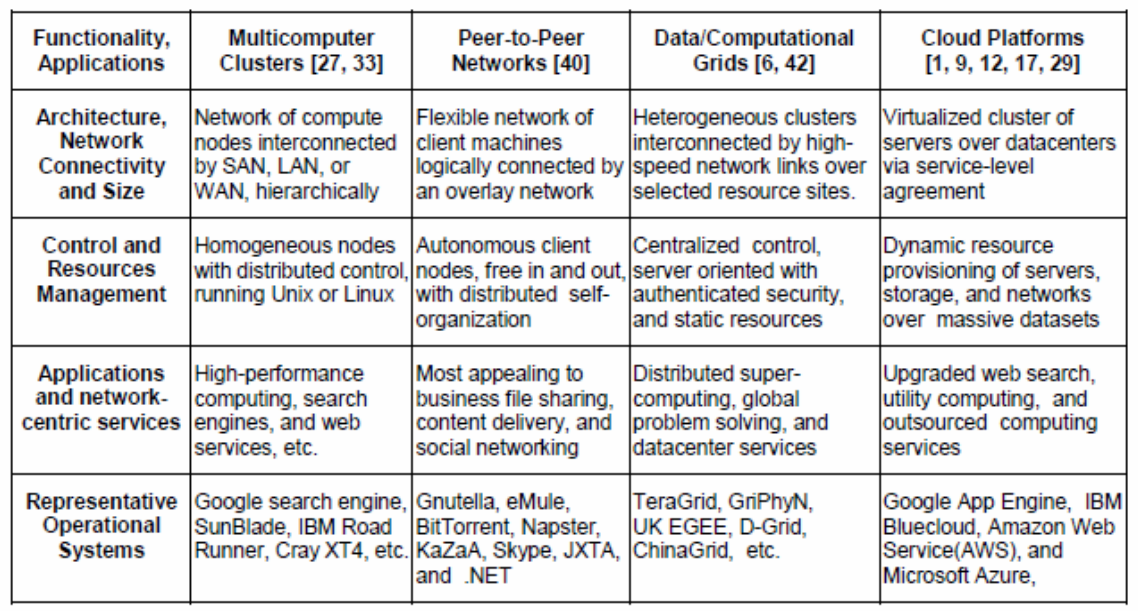
\includegraphics[width=0.9\textwidth]{classification.png}
      \caption{Classification of Distributed Parallel Computing Systems \cite{mainbook}}
       \label{classifictaion}
\end{figure} 

\section{Design principles of clusters}
%Main design objectives of clusters are scalability, packaging, control, homogeneity and security.

\subsection{Scalability}
Single-System Image (SSI). Cluster is used and seen as a single computer with multiply processes and resources. They are used with single interface and can be accessed from any node. Node is a participating computer (physical or virtual). The users aren't aware of the location of physical devices, they agreed to shared all resources to cluster.
We distinguish 3 types of nodes, from point of view of process P:
\begin{itemize}
\item Home node - node where the process P was created.
\item Local node - node on which process P is currently running, process was migrating.
\item Remote nodes - remaining nodes of cluster.
\end{itemize}
Single-System Image is created from many parts which we will further explain:
\begin{itemize}
\item \textbf{Single file hierarchy}

      Can be imagined as "single huge" file system image, that integrates local and global disk of all other devices.
      The functionality of a single file hierarchy have already been partially provided by existing distributed file system in Figure \ref{singlehier}. On this figure we use stable storage.
      \begin{figure}[ht]
      \centering
           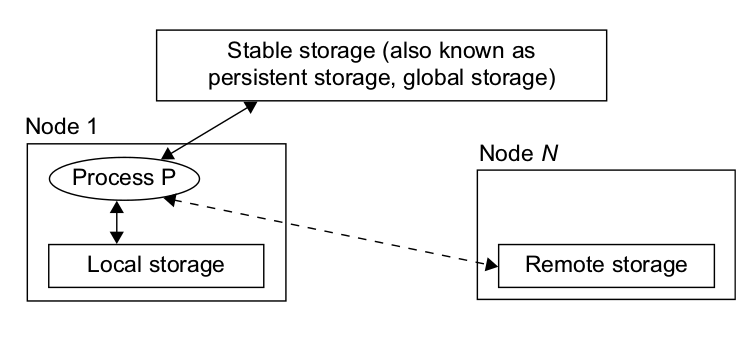
\includegraphics[width=0.7\textwidth]{singlehier.png}
            \caption{Three types of storage in a single file hierarchy. Solid lines show what process P can access and the
      dashed line shows what P may be able to access.}
             \label{singlehier}
      \end{figure} 
\item \textbf{Single point of control}

		System administrator can configure, control, monitor and test all the clusters from single point through protocol SNMP.

\item \textbf{Single entry point}

      Is very rich concept, consisting of single entry point, single file hierarchy, single I/O, etc. It enables users to log to a cluster as one virtual host, although the cluster may have multiply physical host nodes to serve the login session, for example through Telnet, HTTP, etc.

      In cluster as Figure \ref{singleentry} illustrates, is shown how DNS translates the symbolic name and return IP address of the least loaded node, which happen to be \textit{Host1}. Only one user is shown, thousand of users can connect to the cluster in the same fashion. 
      \begin{figure}[ht]
      \centering
           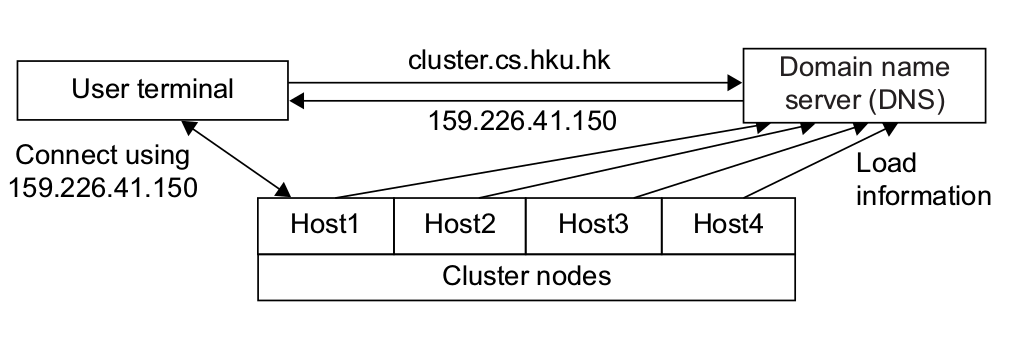
\includegraphics[width=0.7\textwidth]{singleentry.png}
            \caption{Realizing a single entry point in cluster using DNS}
             \label{singleentry}
      \end{figure} 
\item \textbf{Single I/O space}

      Implemented over distributed RAID, shown on Figure \ref{singledisk}. Four node linux cluster with three disks attached to SCSI bus of each node. All PCs can access both local and remote disks. The addressing scheme for all disk blocks is interleaved. \ref{}
      \begin{figure}[ht]
      \centering
           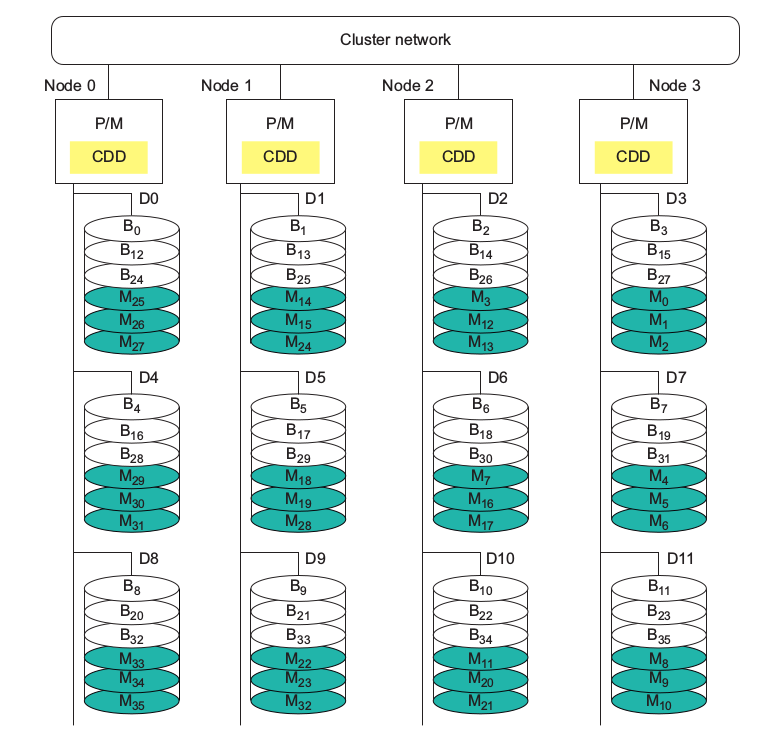
\includegraphics[width=0.6\textwidth]{singledisk.png}
            \caption{Distributed RAID architecture with a single I/O space over 12 distributed disks attached to 4 host computers
      in the cluster}
             \label{singledisk}
      \end{figure} 
\item \textbf{Single networking}

		Any node of the cluster can use any network or I/O device as it were attached to the node which applied for it.

\item \textbf{Single job management}

		All cluster jobs can be submitted from any node to a single
job management system.

\item \textbf{Single memory space}

		As show on Figure \ref{singlemem}, gives user illusion of a big, centralized main memory, which in reality may be clusters. A good way to test if a cluster has a single memory space is to run a sequential program that needs a memory space larger than any single node can provide.

      \begin{figure}[ht]
      \centering
           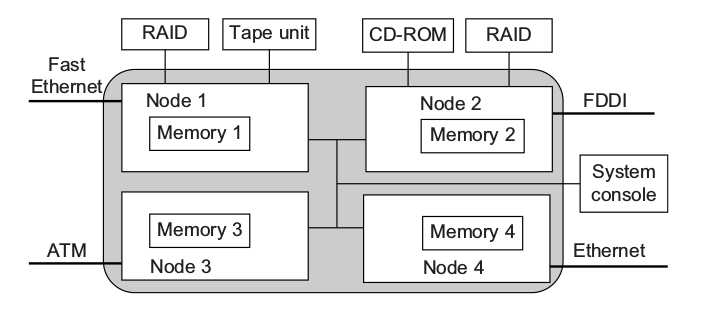
\includegraphics[width=0.6\textwidth]{singlemem.png}
            \caption{A cluster with single networking, single I/O space, single memory, and single point of control.}
             \label{singlemem}
      \end{figure} 		

\item \textbf{Single process space}

		All user processes created on various nodes form a single process space
and share a uniform process identification scheme.

\end{itemize}

\subsection{High-Availability (HA) capability}
High-availability clusters also know as fail-over clusters try to utilized and support server applications with minimum amount of down-time, by using high availability software (we discussed availability in part \ref{MTTF}).

As failure we understand event that prevents the system from normal operation, which can be unplanned or planned and temporarily permanent. Failure can be caused by hardware error, OS crash, bad upgrades, etc.

Possible fault-tolerant cluster configurations:
\begin{itemize}
\item \textbf{Hot standby server clusters}

		Only primary node doing useful work, other node are in standby mode and waiting if primary node fails to continue the work, then replace it from stand-by mode.
\item \textbf{Active-takeover clusters}

		Two nodes are primary, and do useful work, when one fails other take over the work.
\item \textbf{Failover clusters}

		When component fails, the reaming system take over the services of originally failed component.
\end{itemize}

After necessary fault, system have to recover. This recovery process take some time and is usually led by recovery schemes, which are planned before the possible fault, to prepare system and procedures for possible fault. Also checkpoints are used after significant running milestones to make fault recovery easier, by saving the state of the system at some significant points of computation.

%Without shared disks, checkpoints, rollback recovery, failover, and failback are not possible in a cluster.

\section{Massively Parallel Processing (MPP)}
Massively Parallel Processing is the use of many processors to perform a set of coordinated computations in parallel. Traditional MPP machines are distributed memory machines that use multiple processors.

\begin{figure}[ht]
\centering
     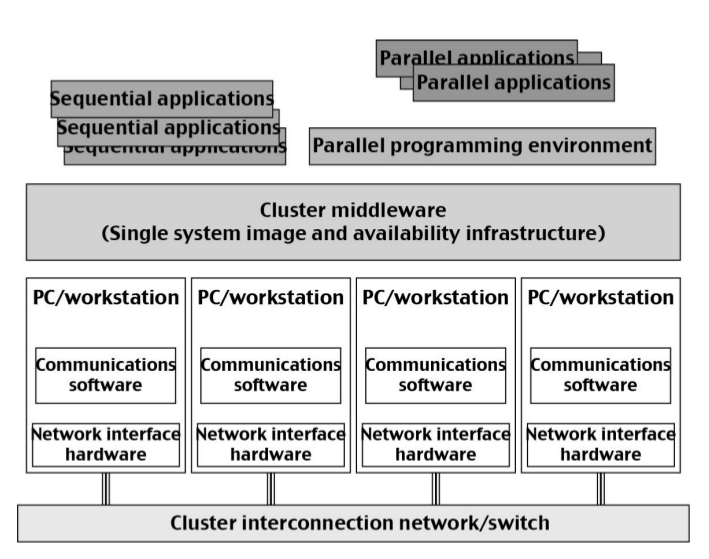
\includegraphics[width=0.7\textwidth]{mpp.png}
      \caption{Example of MPP cluster}
       \label{mpp}
\end{figure} 

As we can see in Top 500 \cite{top500}, MPP machines are only potential opponent to Clusters in nowadays supercomputing. Most know MPP Clusters applications are IBM Blue Gene and Google search engine.

All these system are based on InfiniBand Architecture, point to point. Based on switches, connected through Internet by Host Channel Adapters (HCA) and Target Channel Adapters (TCA).

Cluster can be connected in three ways. Through most common LAN such as Ethernet network, shared disk or SCI bus. The shared-nothing architecture is used in most clusters, where the nodes are connected through the I/O bus. The shared-disk architecture is in favor of small-scale availability clusters in business applications. When one node fails, the other node takes over.

\section{Job Scheduling Methods}
Cluster jobs may be scheduled to run at a specific time (calendar scheduling) or when a particular event happens (event scheduling). Table \ref{jobshedule} summarizes various schemes to resolve job scheduling issues on a cluster. Jobs are scheduled according to priorities based on submission time, resource nodes, execution time, memory, disk, job type, and user identity. With static priority, jobs are assigned priorities according to a predetermined, fixed scheme. The simplest scheme of job scheduling is to schedule jobs in a first-come, first-serve fashion.

\begin{figure}[ht]
\centering
     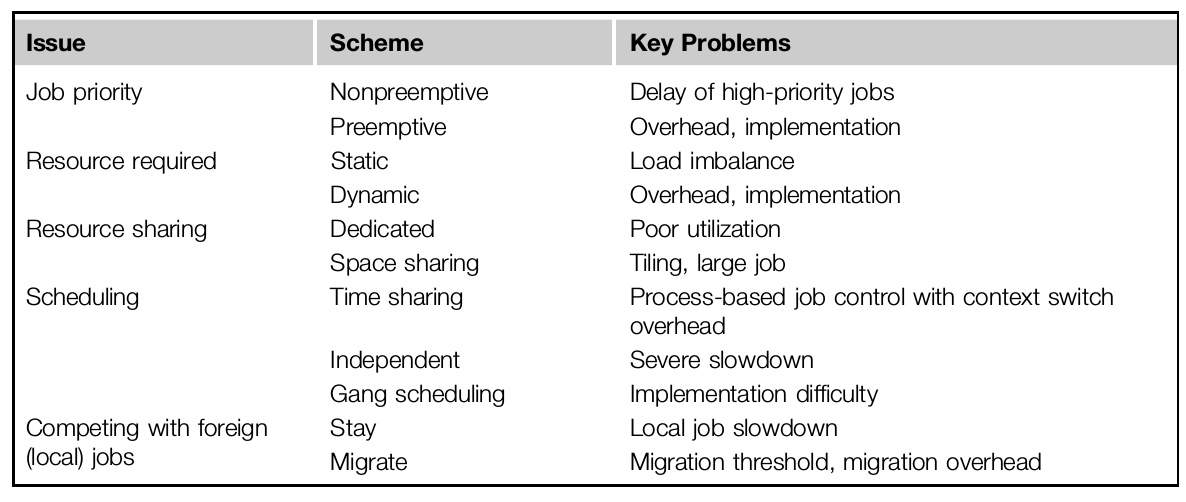
\includegraphics[width=0.9\textwidth]{jobshedule.png}
      \caption{Job scheduling issues and schemes for cluster nodes}
       \label{jobshedule}
\end{figure} 

\chapter{Virtualization}

\section{Virtual Machines}
Virtual Machine (VM) is an emulation of a computer system. They are based on computer architectures and provide functionality of a physical computer. Their implementation may involves special hardware, software or both.

Virtual Machines are divided to three types (as display in Figure \ref{vm}):
\begin{itemize}
\item Native Virtual Machine - Virtual Machine Monitor (VMM) over the Hardware
\item Hosted Virtual Machine - hosting operating system over the hardware
\item Dual-mode Virtual Machine	
\end{itemize}

\begin{figure}[ht]
		\centering
           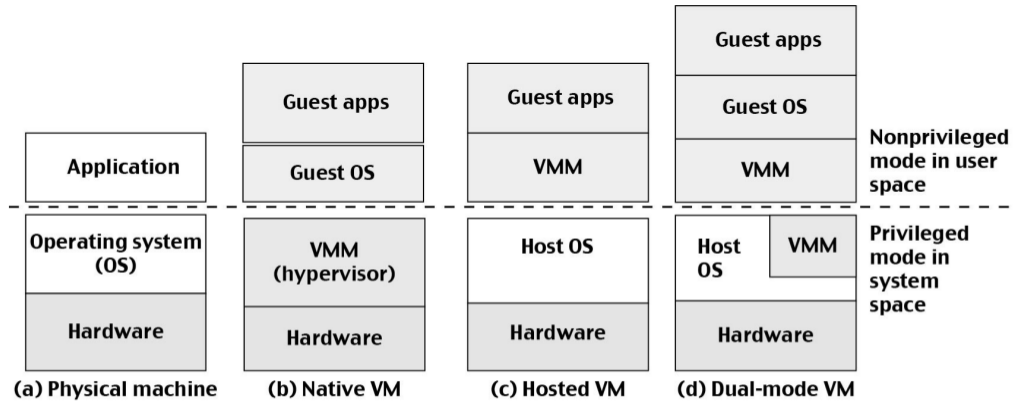
\includegraphics[width=0.8\textwidth]{vm.png}
         \caption{Native, Hosted and Dual-mode VM}
         \label{vm}
\end{figure} 

\subsection{Hypervisor Architecture}
A hypervisor or Virtual Machine Monitor (VMM) is computer software, firmware or hardware that creates and runs virtual machines. A computer, on which a hypervisor runs one or more virtual machines is called a host machine. Hypervision provides hypercalls to guest-OSs and apps. We distinguish two VMM types: microkernel and monolithic.

Dynamic binary translation is the process of converting an executable binary, compiled for a particular ISA into an executable binary for a different ISA at runtime of the executable. This enables transparent execution of a binary compiled for a particular architecture on a different architecture, with no need to modify guest-OS. Done by instruction with two types: critical and non-critical.

Virtual Machine Monitor provides an abstraction identical to the physical machine, so the OS can just run over it as would run on physical hardware. VMM provides low level operations:
\begin{itemize}
\item multiplexing sever of VMs over the same hardware
\item suspension of VM to storage
\item re-suspend VM from hardware
\item VM migration to different hardware
\end{itemize}

If hardware can be virtualized, than all the software environments can be also virtualized. For exmaple as Software as a Service (SaaS), which will be discussed in Chapter \ref{chap:clouds}. \\
\newline
Abstraction levels of virtualization can be divided to 5 parts.
\begin{itemize}
\item \textbf{Instruction System Level (ISA) -}
		Allows to keep running legacy code in legacy hardware.
\item \textbf{Hardware level -}
		On the top of the hardware we can generate virtual hardware. Software layer between hardware and OS. Done by Virtual Machine Monitor (VMM), which require complete control of the system resources. VMM is responsible for allocating all resources. VMM must be efficient, so programs suffer only minor decreasing in speed. Hardware virtualization may be slow, because it creates OS images from scratch.
\item\textbf{ Operating system level -}
		The same as in HW, can be done on top of OS. Also used for cloud based virtualization. OS virtualization insert a virtualization level inside the OS.
\item \textbf{Library support level -}
		Emulator can run windows applications, on UNIX host by using the same API.
\item\textbf{ Application level -}
		For example Java virtual machine
\end{itemize}

\subsection*{Virtualization layer}
Virtualization layer allows multiple customers to be housed on the same physical server with each client having a “private” area on the server to which critical resources are assigned. The performance of one customer’s site does not impact the performance of other sites in a different partition. Also, the number of private areas on each server are limited, ensuring that resources are not over-leveraged.

Types of virtual architectures:
\begin{itemize}
\item Hypervision - between HW and guest-OS
\item Para-virtualization - also between HW and guest-OS, but compiler help in speeding-up by bypassing the VMM
\item Host-based virtualization - VMM on top of the host-OS
\end{itemize}

\subsection*{Para-virtualization}
Para-virtualized VM provides special APIs requiring substantial OS modifications in user applications. Para-virtualization needs to modify the guest operating systems. Performance degradation is a critical issue of a virtualized system. The virtualization layer can be inserted at different positions in a machine soft-ware stack. Figure \ref{paravirt} illustrates the concept of a para-virtualized VM architecture. The guest operating systems are para-virtualized.

\begin{figure}[ht]
		\centering
           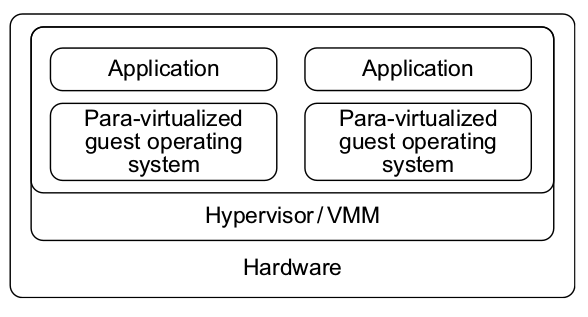
\includegraphics[width=0.5\textwidth]{paravirt.png}
         \caption{Para-virtualized VM architecture, which involves modifying the guest OS kernel to replace nonvirtualizable instructions with hypercalls for the hypervisor or the VMM to carry out the virtualization process}
         \label{paravirt}
\end{figure} 

Hardware support for virtualization or hardware-assisted virtualization is a platform virtualization approach that enables efficient full virtualization using help from hardware capabilities, primarily from the host processors. Full virtualization is used to simulate a complete hardware environment, or virtual machine.

\subsection*{CPU Virtualization}

CPU virtualization involves a single CPU acting as if it were multiple separate CPUs. The most common reason for doing this is to run multiple different operating systems on one machine. CPU virtualization emphasizes performance and runs directly on the available CPUs whenever possible. The underlying physical resources are used whenever possible and the virtualization layer runs instructions only as needed to make virtual machines operate as if they were running directly on a physical machine. VMM runs in supervisor mode. Hardware resources can help in CPU virtualization.

CPU virtualization is not the same thing as emulation. With emulation, all operations are run in software by an emulator. The emulator emulates the original computer’s behavior by accepting the same data or inputs and achieving the same results.

\subsection*{Virtualization of memory}
In a traditional execution environment, the operating system maintains mapping of virtual memory to machine memory with using page tables, which is a one-stage mapping from virtual memory to machine memory. However, in a virtual execution environment, virtual memory virtualization involves sharing the physical system memory in RAM and dynamically allocating it to the physical memory of the VMs. That means a two-stage mapping process should be maintained by the guest OS and the VMM,
respectively: virtual memory to physical memory and physical memory to machine memory. The guest OS continues to control the mapping of virtual addresses to the physical memory addresses of VMs. But the guest OS cannot directly access the actual machine memory. The VMM
is responsible for mapping the guest physical memory to the actual machine memory as in show in Figure \ref{virtmem}.

\begin{figure}[ht]
		\centering
           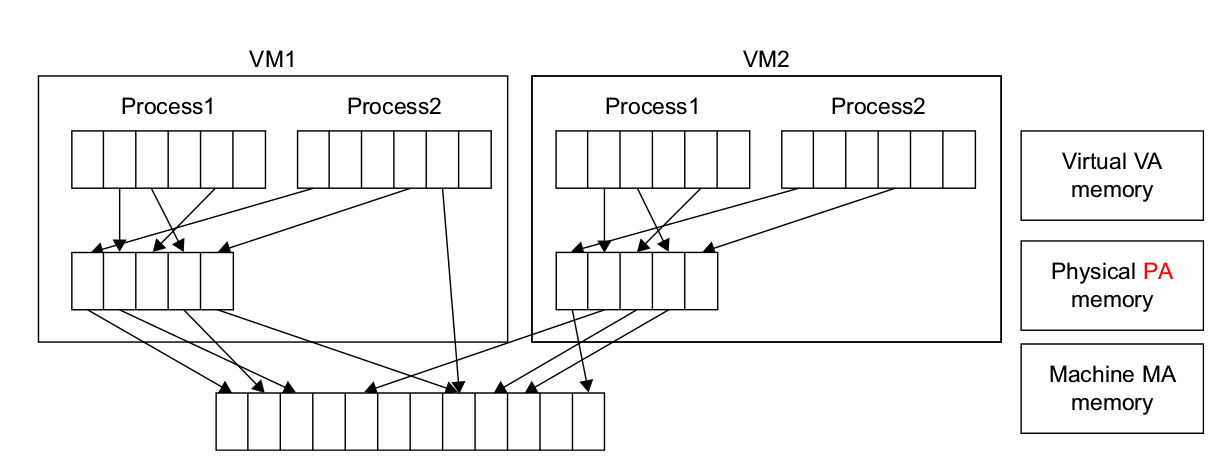
\includegraphics[width=0.9\textwidth]{virtmem.png}
         \caption{}
         \label{virtmem}
\end{figure} 

\subsection{Virtualization of Input/Output (I/O)}
I/O virtualization involves managing the routing of I/O requests between virtual devices and the shared physical hardware. A single hardware device can be shared by multiple VMs that run concurrently. 

\begin{itemize}
\item \textbf{I/O Para-virtualization -}
		Each driver is divided to two parts, front-end which manages requests from guest-OS and back-end which manage the real I/O devices.
\item \textbf{Direct I/O -}
		VMs use directly the I/O device, which work the best with networking devices. That requires hardware support.
\end{itemize}

\subsection*{Physical vs. virtual cluster}
Virtual clusters in contrast with physical clusters are formed with physical machines or a VM hosted by multiple physical clusters. Provisioning VMs to a virtual cluster is done dynamically:
\begin{itemize}
\item Multiple VMs with different OSs can be deployed to the same physical node.
\item Guest-OS can be different from host-OS where VM is implemented.
\item VMs can be replicated in multiple physical servers.
\item Number of nodes of virtual clusters may dynamically vary.
\item Failure of a VM will not put down the host system.
\end{itemize}

\subsection*{Virtual machines fast deployment and scheduling}
Deployment is construct of software stacks as OS, libraries and applications. Quickly switching between virtual clusters to use of resources at highest efficiency.
Automatic scale-up/scale-down based on load balancing are big advantage of virtualization and increase resource utilization and reduces response time.
High performance virtual storage is necessary for efficient VM deployment.
Process of deployment of VM in cluster:
\begin{itemize}
\item Prepare disk image.
\item Configure VM.
\item Choose destination nodes.
\item Execute VM deployment command on every host.
\end{itemize}

\subsection{Live VM migration}
Process of moving a \underline{running} virtual machine or application between different physical machines without disconnecting the client or application is called live VM migration. Memory, storage and network connectivity is also transferred from original machine to the destination.

Main purpose of migration is enhance fail-over flexibility. When a VM fails, new VM replace it in the same or different host. In case of host failure, VM live migration allows the service to survive.

Virtual machine can be situated in 4 states: \textit{inactive} (not enabled), \textit{active} (performing a real task), \textit{paused} (waiting), \textit{suspended} (resources stored back to the disk).

Methods of virtual clusters migration:
\begin{itemize}
\item Guest-based manager - manager resides on a guest-OS.
\item Host-based manager - manager is situated in actual physical node, in the host, when is supervising the VMs.
\item Independent manager - uses both, guest and host.
\item Integrated cluster - distinguishes between virtualized and physical resources.
\end{itemize}

Memory, files and network resources can be also migrated. Memory migration must be done efficiently from small to big sizes. Files system migration can be done in two solutions. As one virtual disk for each VM, contains file system or as global file system across all VMs. Network migration must maintain all open network connections, assign and keep virtual IP. In the manner we have to also need to have in mind, as in classic network UDP connection, that some packets may be lost.

\subsection*{Data centers}

Server consolidation in data center is an approach to the efficient usage of computer server resources in order to reduce the total number of servers or server locations that an organization requires. The practice developed in response to the problem of server sprawl, a situation in which multiple, under-utilized servers take up more space and consume more resources than can be justified by their workload.

Virtual storage management means, that each of the running programs can assume, that it has access to all of the storage, defined by the architecture's addressing scheme. The only limit is the number of bits in a storage address. This ability to use a large number of storage locations is important because a program may be long and complex, and both the program's code and the data it requires must be in central storage for the processor to access them.

Data centers must be virtualized to serve as a cloud providers. For this task we use Virtual Infrastructure (VI). VI create VM and aggregate it into virtual cluster as a elastic resource. For this purpose we usually use OpenStack. OpenStack is a set of software tools for building and managing cloud computing platforms for public and private clouds.

Because of VMM can change the computer architecture, means a SW layer between HW and VMs. VM encapsulates the state of the guest OS running on it, this is a security problem. VMM provides the security isolation needed by VMs, but once a attacker successfully enters a VMM, they have whole system of VM.
By danger of this we create VM-based intrusion detection. By intrusion is mean unauthorized access to computer, OSs build on characterizing disreputable actions, etc. 

\chapter{Clouds} \label{chap:clouds}
Cloud architectures are built with commodity hardware and network (WSC). Design emphasize performance/price ratio instead of only performance. Clouds promises much more than data center model.
Three types of clouds:
\begin{itemize}
\item \textbf{Public cloud}

			A public cloud is basically the internet. Service providers use the internet to make resources, such as applications (also known as Software-as-a-service) and storage, available to the general public, or on a public cloud. Owned by the service providers, which are responsible for creating and managing of VM within their infrastructure.
\item \textbf{Private cloud}

			Private clouds are data center architectures owned by a single company that provides flexibility, scalability, provisioning, automation and monitoring.  The goal of a private cloud is not sell “as-a-service” offerings to external customers, but instead to gain the benefits of cloud architecture without giving up the control of maintaining your own data center.
\item \textbf{Hybrid cloud}

			By using a Hybrid approach, companies can maintain control of an internally managed private cloud while relying on the public cloud as needed.  For instance during peak periods individual applications, or portions of applications can be migrated to the Public Cloud.  This will also be beneficial during predictable outages: hurricane warnings, scheduled maintenance windows, rolling brown/blackouts.
\end{itemize}

\begin{figure}[ht]
		\centering
           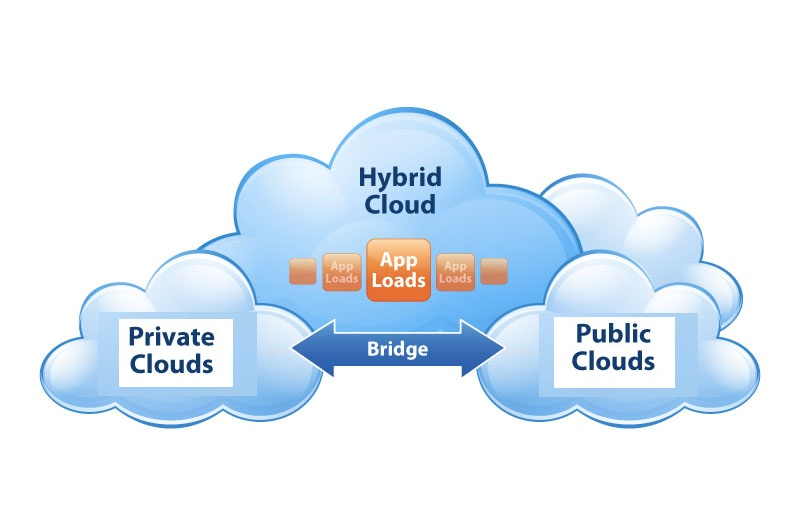
\includegraphics[width=0.9\textwidth]{cloud.png}
         \caption{Three types of cloud, private, public and hybrid between them.}
         \label{cloud}
\end{figure} 

Clouds are based on the paradigm that user pay-per-use of service. Based on subscription and quality of service. That is the principal cost reducer of cloud services. The mainly design objectives are shifting computing from desktops to data centers, service provisioning, scalability in performance, data privacy protection, hight quality of cloud service, new standards and interfaces. 

Three types of cloud application services:
\begin{itemize}
\item \textbf{IaaS}

			Infrastructure as a Service are self-service models for accessing, monitoring, and managing remote datacenter infrastructures, such as compute (virtualized or bare metal), storage, networking, and networking services (e.g. firewalls). Instead of having to purchase hardware outright, users can purchase IaaS based on consumption, similar to electricity or other utility billing. Users can control over OS, deploy and run apps as virtualizing resources.
\item \textbf{PaaS}

			Platform as a Service are used for applications, and other development, while providing cloud components to software. Built on the top of IaaS. What developers gain with PaaS is a framework they can build upon to develop or customize applications. PaaS makes the development, testing, and deployment of applications quick, simple, and cost effective. With this technology, enterprise operations, or a third-party provider, can manage OS's, virtualization, servers, storage, networking, and the PaaS software itself. Developers, however, manage the applications. User can use programing languages and software tools provide by cloud.
\item \textbf{SaaS} 

			Software as a Service represent the largest cloud market and are still growing quickly. Built on the top of PaaS. SaaS uses the web to deliver applications that are managed by a third-party vendor and whose interface is accessed on the clients side. Most SaaS applications can be run directly from a web browser without any downloads or installations required, although some require plugins. User don't have to invest in server or software providers, just in stored data. Providers can keep very low costs.
\end{itemize}

\section{Warehouse-Scale Data-Center design}
As computation continues to move into the cloud, the computing platform of interest no longer resembles a pizza box or a refrigerator, but a warehouse full of computers. These new large datacenters are quite different from traditional hosting facilities of earlier times and cannot be viewed simply as a collection of co-located servers. Large portions of the hardware and software resources in these facilities must work in concert to efficiently deliver good levels of Internet service performance, something that can only be achieved by a holistic approach to their design and deployment. In other words, we must treat the datacenter itself as one massive warehouse-scale computer (WSC).

Clouds work on massive data centers up to one million servers. By the size of data-center we can lower the cost of unit, but with size, we still must ensure cooling, sufficient network bandwidth and also deal with hardware/software failures.

Very import part of making a good working data center is ensure good work of data center interconnection network, which can be sum up to five requirements:
\begin{itemize}
\item low latency
\item high bandwidth
\item low cost
\item message-passing interface
\item fault-tolerance
\end{itemize}

The network topology should support all message-parsing interface (MPI) communication patterns. Both point-to-point and collective MPI communications must be supported. The network should have high bisection bandwidth to meet this requirement.

The interconnection network should be expandable. With thousands or even hundreds of thousands of server nodes, the cluster network interconnection should be allowed to expand once more servers are added to the data center.

The interconnection network should provide some mechanism to tolerate link or switch failures. In addition, multiple paths should be established between any two server nodes in a data center. Fault tolerance of servers is achieved by replicating data and computing among redundant servers.

\begin{figure}[ht]
		\centering
           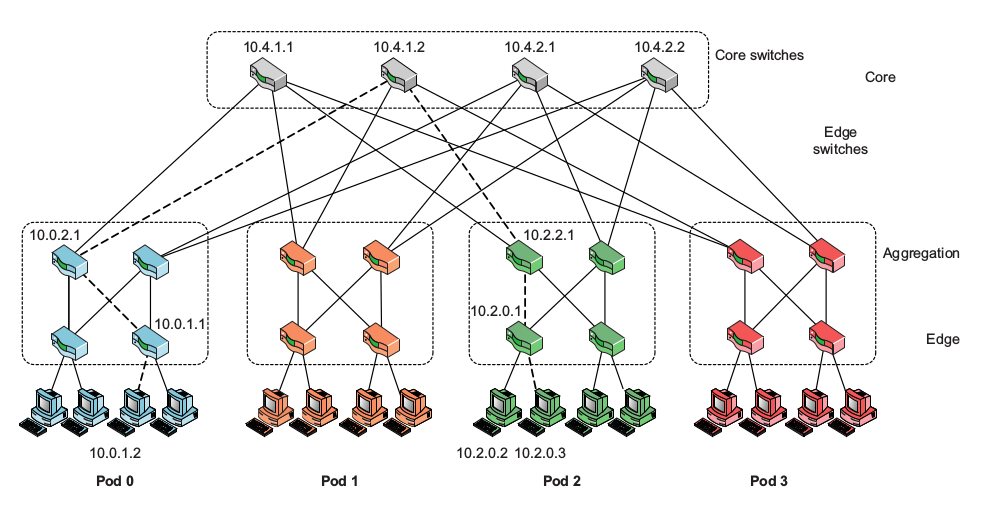
\includegraphics[width=0.9\textwidth]{centerconn.png}
         \caption{A fat-tree interconnection topology for scalable data-center construction.}
         \label{centerconn}
\end{figure} 

\section{Layered cloud architectural development}
Cloud development architecture is divided to three layers:
\begin{itemize}
\item \textbf{Infrastructure layer}

			The basic layer of Cloud is the infrastructure IaaS. This layer is basically hardware and network. What distinguishes this from a regular server or hosting company are mainly two things, scalability and virtualization.
\item \textbf{Platform layer}

			The second layer of Cloud is the platform – the PaaS. The platform layer provides resources to actually build applications. In combination with IaaS, PaaS provides the ability to develop, test, run and host applications. The platform layer opens up for 3. parties to add their software (or integrations) to a Cloud service.
\item \textbf{Service layer}

			The third Cloud layer is the actual Software – the SaaS. SaaS has been used for many years, but in a Cloud setting it is the layer in which the user consumes the offering from the service provider. The SaaS layer must be web based and hence accessible from everywhere and preferably on any device.
\end{itemize}

\begin{figure}[ht]
		\centering
           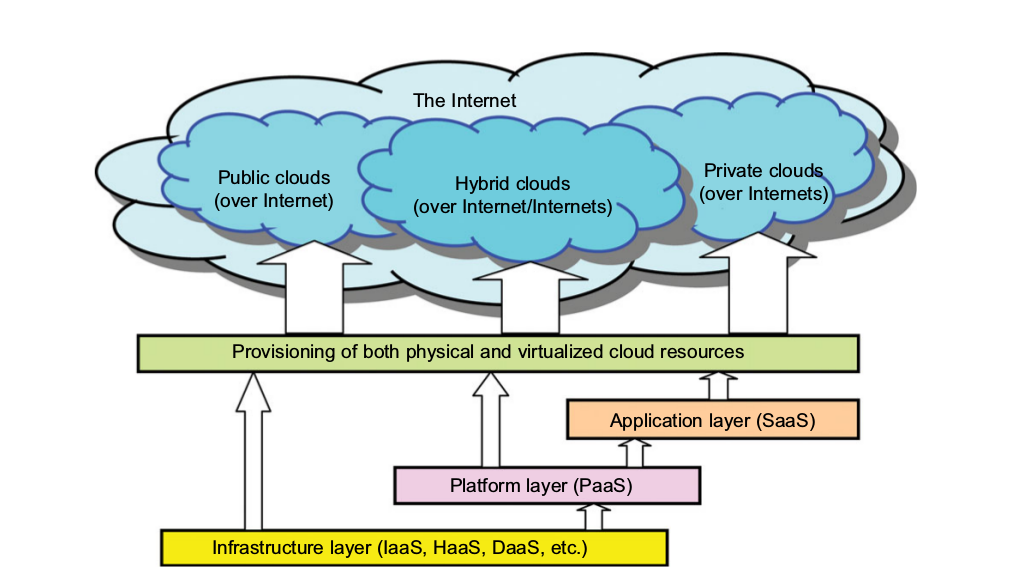
\includegraphics[width=0.9\textwidth]{cloudlayers.png}
         \caption{Layered architectural development of the cloud platform for IaaS, PaaS, and SaaS applications over the
Internet.}
         \label{cloudlayers}
\end{figure} 

\subsection*{Virtualization support for the Cloud}
One very distinguishing feature of cloud computing infrastructure is the use of system virtualization and the modification to provisioning tools. Virtualization of servers on a shared cluster can consolidate web services. As the VMs are the containers of cloud services, the provisioning tools will first find the corresponding physical machines and then deploy the VMs to those nodes before scheduling the service to run on the virtual nodes.

In many cloud computing systems, virtualization software is used to virtualize the hardware. System virtualization software is a special kind of software which simulates the execution of hardware and runs even unmodified operating systems. Cloud computing systems use virtualization software as the running environment for legacy software such as old operating systems and unusual applications. It's give extremely flexibility to users, as they have fill privileges on their systems and also they have complete isolation.

\subsection{Challenges of architectural design}
Some of promising challenges in cloud design:
\begin{itemize}
\item \textbf{Service availability}

			Single company can cause single point of failure even in many of their data centers at once.
\item \textbf{Data privacy and security}

			Public clouds are exposed to attack, as every user have access. They are vulnerable to classic network attacks as DoS, malware, worm etc. But also to cloud attacks as man-in-the-middle, hyper-vision malware, etc. This can be secure by encrypted storage, virtual LAN, network security as firewall etc.
\item \textbf{Unpredictable performance}

			Mostly cause by I/O, by sharing them, which can cause conflicting between other applications or VM's. Solution is to virtualize disks, introduce interrupts etc.
\item \textbf{Software bugs}

			Debugging large scale distributed bugs is difficult, because it cannot be reproduced. Virtualization can capture information very important for debugging.
\item \textbf{Scalability, interoperability, standardization}

			Pay-as-you-go for computing is difficult.
\item \textbf{Software licensing}

			Open source software is used because licensing is much better. Traditional software supplier must adapt to cloud model.
\end{itemize}

\subsection{Cloud security}

Trust and security are key to gain the confidence of providers and users. A healthy cloud ecosystem is desired to free users from abuses, violence, cheating, hacking, viruses,
rumors, pornography, spam, and privacy and copyright violations. 
Three basic cloud security enforcements are expected:
\begin{itemize}
\item Facility security - Security of building which store cloud servers. Access restrictions, alarms, man traps, etc.
\item Network security - Fault tolerant external firewalls, vulnerability assessment, etc.
\item Platform security -SSL, data encryption, password policies, etc.
\end{itemize}

Virtualization enhances cloud security. But VMs add an additional layer of software that could become single point of failure. Security attacks in one VM are isolated and contained from affecting the other VMs. The Figure \ref{cloudsec} lsit eight protection schemes to secure clouds and data centers.

\begin{figure}[ht]
		\centering
           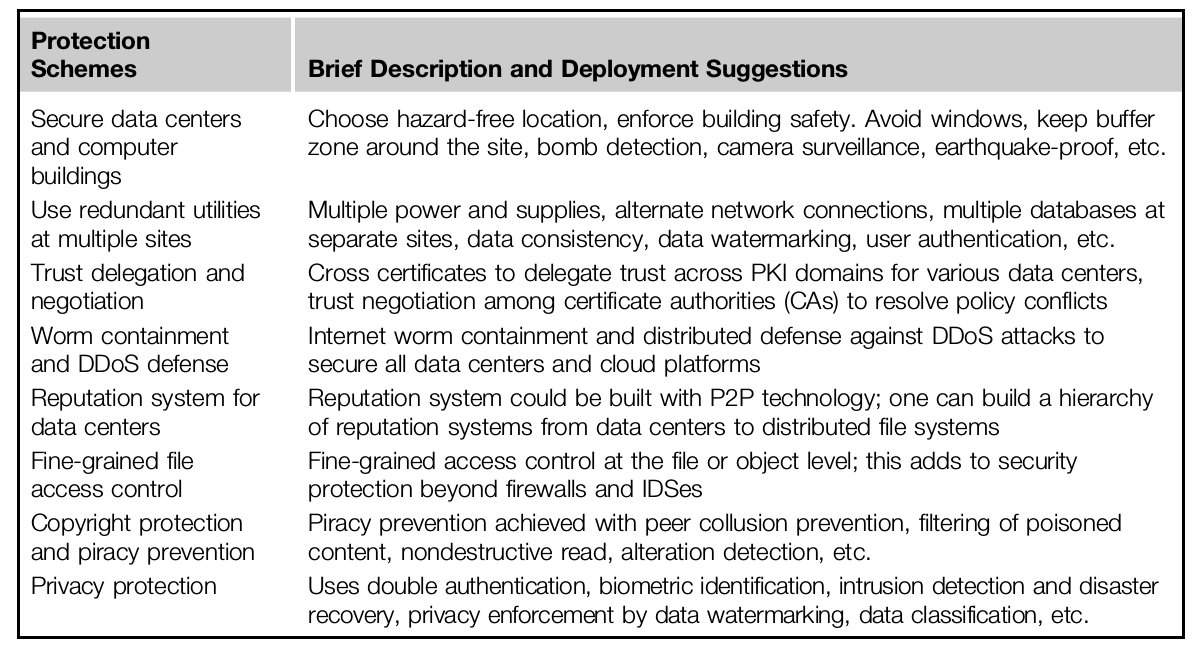
\includegraphics[width=0.99\textwidth]{cloudsec.png}
         \caption{Physical and Cyber Security Protection at Cloud/Data Centers.}
         \label{cloudsec}
\end{figure} 

\subsection*{Distributed intrusion/anomaly detection}

Data security is the weakest link in all cloud models. We need new cloud security standards to apply common API tools to cope with the data lock-in problem and network attacks or abuses.
Security threats may be aimed at VMs, guest OSes, and software running on top of the cloud. IDSes attempt to stop these attacks before they take effect.

\begin{itemize}
\item \textbf{Distributed Defense against DDoS Flooding Attacks}

		A DDoS defense system must be designed to cover multiple network domains spanned by a given cloud platform. These network domains cover the edge networks where cloud resources are connected. DDoS attacks come with widespread worms.
        
\item \textbf{ Man in the middle attack}

Migration from host A to host B via security vulnerable network. The man in the middle can view the VM contents being migrated, steal data and modify VM contents.		

\end{itemize}

\subsection*{Data and software protection techniques}
\begin{itemize}
\item \textbf{Data integrity and privacy protection}

		Users desire a software environment that provides many useful tools to build cloud applications over large data sets. In addition to application software, users need some security and privacy protection software for using the cloud. Such software should offer special APIs, fine-grained access control, protected shared data sets, personal firewalls, etc.
        
\item \textbf{Data coloring and cloud watermarking}

		With shared files and data sets, privacy, security, and copyright information could be compromised in a cloud computing environment. Users desire to work in a trusted software environment that provides useful tools to build cloud applications over protected data sets. The user identification is also colored to be matched with the data colors. This color matching process can be applied to implement different trust management events.
\end{itemize}


%%%%%%%%%%%%%%%%
% Bibliography %
%%%%%%%%%%%%%%%%
\begin{thebibliography}{9}
\bibitem{mainbook} 
Kai Hwang, Jack Dongarra, Geoffrey C. Fox.
\textit{Morgan Kauthann}. (English) 
[\textit{Distributed and Cloud Computing: From Parallel Processing to the Internet of Things}]. 
Annalen der Physik, ISBN-13: 978-0123858801.

\bibitem{htcondor} 
Computing with HTCondor™,
\\\texttt{https://research.cs.wisc.edu/htcondor/htc.html}

\bibitem{nvidia} 
Main website of NVidia™,
\\\texttt{https://www.nvidia.com/object/what-is-gpu-computing.html}

\bibitem{top500} 
TOP500 Supercomputer Sites,
\\\texttt{https://www.top500.org/lists/2017/11/}

\end{thebibliography}

\end{document}